\chapter{Metodika}


%V této části buďte velmi precizní. Vše musíte popsat tak důkladně, aby kdokoliv mohl vaše pokusy či
%pozorování zopakovat. Nezapomeňte uvést velikost vzorků, věk a pohlaví zvířat, denní a roční dobu,
%podmínky chovu nebo popis lokalit (třeba včetně mapky), specifické přístrojové vybavení
%(pokud je to důležité, např.~pro srovnání výsledků s publikovanými údaji, uveďte i přesný typ
%přístroje) a jiné podrobnosti. Také může být dobré zmínit, jak jste zabránili vlivu pakovaného testování stejných
%individuí a proč se domníváte, že je počet jedinců dostatečný k zodpovězení vašich otázek. Více než
%vhodné je zmínit a zdůvodnit použité statistické metody a počítačové programy. Používáte-li zkratky, uveďte
%jejich seznam.
%Materiál a metodika bývají pro větší srozumitelnost často členěny na menší podkapitoly: materiál,
%experimentální design, analýza dat atd. Systém více podkapitol třeba jen o třech řádcích bývá přehlednější
%než souvislý odstavec na dvě strany. (A to samozřejmě neplatí jen pro metodiku.)
%Čtení DP usnadní, pokud je členění na podkapitoly obdobné v kapitolách Materiál a metodika,
%Výsledky a případně i Diskuse.
%Při vší pečlivosti se však snažte být poměrně struční. Materiál a metodika by neměly tvořit většinu DP.

XXX neco trosku obecnejsiho?

\section{Simulace}

\begin{figure}[h]
    \centering

    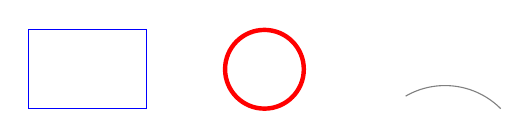
\begin{tikzpicture}
        \draw [blue] (0,0) rectangle (1.5,1);
        \draw [red, ultra thick] (3,0.5) circle [radius=0.5];;
        \draw [gray] (6,0) arc [radius=1, start angle=45, end angle= 120];
    \end{tikzpicture}

    \caption{XXX picture: Big picture}
\end{figure}

Použil jsem stochastický model postavený na individuích. Individua jsou jedinci jednoho druhu. Mají rozlišená
dvě pohlaví. Jejich populace je panmiktická -- žijí v nestrukturovaném prostředí, kde jejich rozložení v prostoru nemá
vliv na pravděpodobnost jejich křížení a tvorba párů je náhodná a nezávisí ani na jejich příbuznosti, ani na jejich
fenotypu, ani na jiném faktoru.

Fenotyp jedinců je modelován jako čtyři nezávislé kvantitativní vlastnosti a reprezentován jako čtyřrozměrný vektor.
Prostředí určuje pro modelovaný druh optimální fenotyp. Optimum prostředí, čtyřrozměrný vektor $E(t)$, není stálé,
ale může se měnit v čase.

Euklidovská vzdálenost fenotypu jedince od aktuálního optima prostředí určuje jeho fitness.

Optimum prostředí je po dobu 8192 kroků simulace konstantní a následně dojde k jeho skokové změně o
$\Delta{}E$. Po této změně opět zůstane optimum neměnné po dalších 8192 kroků, poté se vrátí na počáteční hodnotu.

Počáteční velikost populace je jedním z parametrů simulace.  V~dalších krocích je následně velikost populace
udržována dvěma mechanismy - turbidostatickou regulací a umíráním příliš starých jedinců.

Čerstvě narození jedinci jsou sexuálně dospělí ihned v následujícím kroku simulace a věk neovliňuje jejich fenotyp.
Pokud není jedinec odstraněn turbidosatem, tak po 64 krocích umírá stářím.

V každém kroku jsou z populace náhodně vybrány páry opačného pohlaví.
Kolik pár vyvede potomků, je určeno průměrnou fitness páru. Způsob, jak je jsou určeny počty potomků, jejich geny a
jak následně geny určují jejich fenotyp, je popsán později.

Při každém kroku simulace také velmi malou část jedinců postihne mutace jednoho nebo více genů. Tyto mutace mají
vliv na geny, které mohou zdědit potomci jedince, jeho fenotyp však již neovlivňují a ten zůstává konstatní po celou
dobu života. Somatické mutace nejsou modelovány.

\section{Jedinec a jeho geny}

Geny každého jedince jsou uloženy v dvou homologních chromosomech. Každý z těchto chromosomů má 20 lokusů.
Na každém z lokusů je alela, která má vliv na fenotyp jedince. Alela je určena svým příspěvkem k fenotypu (čtyřrozměrný
vektor, typicky s jednou nenulovou hodnotou, tedy gen ovlivňuje jednu vlastnost jedince, dále nazýván i
\textit{efekt alely}) a svým příspěvkem k fenotypu, pokud se vyskytuje ve dvou instancích v témže lokusu
(opět čtyřrozměrný vektor, dále nazýván i \textit{dominantní efekt alely}).

Na počátku simulace je vygenerována populace složená z náhodných jedinců.
Jejich počet je parametrem simulace, zároveň je počáteční velikost populace používána i jako rovnovážná velikost
populace pro její následnou regulaci.

Náhodní počáteční jedinci jsou generováni tak, že jsou pro každého z nich vygenerované náhodné alely, vybráno náhodně
jedno ze dvou pohlaví a na základě toho určen fenotyp.

Jak vypadají náhodně generované alely, je určeno parametry simulace -- mezi nimi je, jaká je pravděpodobnost, že bude
nová alela ovlivňovat více složek fenotypu (je \uv{pleiotropická}) a jaká je pravděpodobnost, že se u alely projeví
dominance.

Pokud alela působí jen na jednu vlastnost, tak je tato vlastnost vybrána náhodně a velikost příspěvku je vybrána z
normovaného normálního rozdělení.\footnote{Pokud mluvím o normálním rozdělení bez dalšího upřesnění, tak mám na mysli
právě normované normální rozddělení se střední hodnotou $0$ a rozptylem $1.0$ tedy $N(0, 1)$}
Pokud působí na všechny složky fenotypu, tak jsou příspěvky vybrány nezávisle na sobě z normálního
rozdělení a vyděleny odmocninou z dimenze fenotypu (tedy konkrétně $\sqrt{4} = 2$).
Důvodem je, že bez tohoto znormování měly pleiotropické příspěvky v průměru větší délku. XXXX vysvetlit

Teorie zamrzlé plasticity předpokládá podstatný význam alel, které působí v opačných směrech, pokud se
v jednom lokusu vyskytnou v jedné nebo ve dvou kopiích (dále jsou tyto alely nazývány pro jednoduchost
\uv{negativně dominantní}).\footnote{
V častém případě je takto ovlivňována přímo fitness jedince. V tomto zjednodušeném modelu předpokládáme, že dané alely
ovlivňují přímo jednotlivé složky fenotypu.
} Pravděpodobnost, že alela má takovou vlastnost, je parametrem simulace.

Ostatní alely mají účinek stejný, ať již jsou na daném locusu na jednom nebo na obou chromosomech.

\begin{tcolorbox}[ title={Pseudokód popisující generování náhodné alely}
                 , breakable
                 ]

\begin{code}[commandchars=\\\{\}]
nahodna_alela() =
    \textbf{pokud} (R(0,1) < pomer_pleiotropickych_alel)
        \textbf{pak}
            efekt <- nahodny_jednoduchy_efekt()
            dominantni_efekt <- nahodny_dominantni_efekt(efekt)
            Alela(efekt, dominantni_efekt)
        \textbf{jinak}
            efekt <- nahodny_pleiotropicky_efekt()
            dominantni_efekt <- nahodny_dominantni_efekt(efekt)
            Alela(efekt, dominantni_efekt)

nahodny_jednoduchy_efekt() =
    zamichej([0, 0, 0, \textit{N}()])

nahodny_jednoduchy_efekt() =
    [\textit{N}() / 2, \textit{N}() / 2, \textit{N}() / 2, \textit{N}() / 2])

nahodny_dominantni_efekt(efekt) =
    \textbf{pokud} (R(0,1) < pomer_negativne_dominantnich_alel)
        \textbf{pak} efekt
        \textbf{jinak} nahodny_opacny_efekt(efekt)

nahodny_opacny_efekt(efekt) =
    x <- P(1.5, 1.5)
    (-x) * efekt \textit{//násobení vektoru (záporným) skalárem}

\textit{// {R}(0, 1) značí náhodné číslo z rovnoměrného rozdělení}
\textit{//           na intervalu (0, 1)}

\textit{// {N}() značí náhodné číslo ze standardizovaného}
\textit{//       normálního rozdělení}

\textit{// {P}(xm, a) značí náhodné číslo z Paretova rozdělení}
\textit{//            s parametry xm a a}
\end{code}
\end{tcolorbox}

\subsection{Křížení}

Každý jedinec má jedno ze dvou pohlaví. V každém kroku simulace jsou náhodně vytvořeny nové páry jedinců opačného
pohlaví. Zda pár přivede na svět nového jedince, závisí na fitness obou potenciálních rodičů mechanismem, který je
popsán později.

Každý z potomků vzniká tak, že jsou rekombinovány geny obou rodičů -- z každého jedince je náhodně vybrán jeden
z chromosomů, je zvolen jeden náhodný locus. Locusy před ním a on jsou naplněny alelami jednoho z rodičů,
lokusy po něm alelami druhého z rodičů, čímž vznikne první chromosom potomka. Druhý chromosom potomka je vytvořen
analogicky -- locusy před zvoleným locusem a on jsou naplněny alelami druhého z rodičů, zbytek chromosomu alelami
prvního rodiče.

Pohlaví potomka je určeno náhodně se stejnou pravděpodobností pro obě pohlaví.

\begin{figure}[h]
  \centering

  \begin{tikzpicture}

    \begin{scope}
      \DNASequence[Parent1a]{$\blacktriangleright$/yellow!30,$\clubsuit$/yellow!30,$\boxplus$/yellow!30,$\circ$/yellow!30,$\circledcirc$/yellow!30,$\flat$/yellow!30}
    \end{scope}

    \begin{scope}[yshift=1cm]
      \DNASequence[Parent1b]{$\triangleright$/yellow!20,$\diamondsuit$/yellow!30,$\boxdot$/yellow!20,$\bullet$/yellow!30,$\circledcirc$/yellow!30,$\flat$/yellow!30}
    \end{scope}

    \begin{scope}[yshift=3cm]
      \DNASequence[Parent2a]{$\blacktriangle$/green!30,$\clubsuit$/green!30,$\boxdot$/green!30,$\star$/green!30,$\circledcirc$/green!30,$\flat$/green!30}
    \end{scope}

    \begin{scope}[yshift=4cm]
      \DNASequence[Parent2b]{$\triangle$/green!20,$\clubsuit$/green!30,$\Box$/green!20,$\ast$/green!30,$\circledcirc$/green!30,$\sharp$/green!30}
    \end{scope}


    \begin{scope}[xshift=9cm,yshift=2cm]
      \DNASequence[Donea]{$\blacktriangleright$/yellow!30,$\clubsuit$/yellow!30,$\Box$/green!20,$\ast$/green!30,$\circledcirc$/green!30,$\sharp$/green!30}
    \end{scope}

    \begin{scope}[xshift=9cm,yshift=3cm]
      \DNASequence[Doneb]{$\triangle$/green!20,$\clubsuit$/green!30,$\boxplus$/yellow!30,$\circ$/yellow!30,$\circledcirc$/yellow!30,$\flat$/yellow!30}
     \end{scope}

    \ConnectNodes[out=-90, in=-30]
        {Donea-1.south west}
        {Parent1a-1.south west};

    \ConnectNodes[out=-90, in=-60]
        {Donea-5.south}
        {Parent2b-5.south east};

    \ConnectNodes[out=90, in=40]
        {Doneb-0.north east}
        {Parent2b-0.north east};

    \ConnectNodes[out=120, in=60]
        {Doneb-5.north}
        {Parent1a-5.north east};

  \end{tikzpicture}

  \caption{Křížení}
\end{figure}


\subsection{Mutace}

Jedinou možnou mutací je bodová změna alely za jinou -- nejsou tedy simulovány rozsáhlejší mutace, které
by měly větší vliv na strukturu DNA.

Nad každým lokusem v obou chromosomech je náhodně s pravděpodobností $0.0002$ rozhodnuto, zda u~něj dojde ke změně.
V~případě, že ano, tak je na lokus dána nově vygenerovaná náhodná alela. Ta je vybírána stejným mechanismem, jako jsou
generovány počáteční alely.

\begin{figure}[h]
  \centering

  \begin{tikzpicture}

    \begin{scope}
      \DNASequence[Mutated]{$\blacktriangleright$/white!30,$\clubsuit$/red!30,$\#$/white!30,$\triangleleft$/white!30,$\circ$/white!30,$\flat$/white!30}
    \end{scope}

    \begin{scope}[yshift=1cm]
      \DNASequence{$\triangleright$/white!20,$\clubsuit$/white!30,$\bot$/white!20,$\triangleleft$/white!30,$\bullet$/white!30,$\sharp$/white!30}
    \end{scope}


    \begin{scope}[xshift=9cm]
      \DNASequence[Done]{$\blacktriangleright$/white!30,$\diamondsuit$/green!30,$\#$/white!30,$\triangleleft$/white!30,$\circ$/white!30,$\flat$/white!30}
    \end{scope}

    \begin{scope}[xshift=9cm,yshift=1cm]
      \DNASequence{$\triangleright$/white!20,$\clubsuit$/white!30,$\bot$/white!20,$\triangleleft$/white!30,$\bullet$/white!30,$\sharp$/white!30}
    \end{scope}

    \ConnectNodes[out=-90, in=-30]
        {Done-1.south}
        {Mutated-1.south};

  \end{tikzpicture}

  \caption{Mutace}
\end{figure}

\section{Jedinec a jeho fenotyp}

Fenotyp jedince jsou jeho čtyři kvantitativní vlastnosti dohromady reprezentované jako čtyřrozměrný vektor.

Každá alela nějak přispívá k výslednému fenotypu, tyto příspěvky (resp. terminologií simulace efekty) se sčítají.
Příspěvek alely se může lišit, pokud se nachází ve dvou kopiích v témže lokusu na obou chromosomech --
v tom případě se použije její dominantní efekt.

Simulace obsahuje možnost namodelovat pohlavní dimorfismus, kdy fenotyp závisí i na pohlaví, ale tato varianta nebyla
v~simulacích studována.

\section{Optimum}

Pro simulovaný druh existuje optimální fenotyp, který nejlépe vyhovuje aktuálnímu stavu prostředí.
Tento optimální fenotyp se v průběhu simulace dvakrát skokově -- v jejím kroku číslo 8192 a 16384 -- změní. Délky
stabilních intervalů jsou zvoleny tak, aby se ve většině simulací populace buď přizpůsobila a jedinci se přiblížili
optimu, nebo vyhynula.

Počáteční optimum je nastaveno na dvanáctinásobek výběru z normálního rozložení nezávisle pro každou dimenzi -- pro
každou složku vektoru je vybráno náhodné číslo z normovaného normálního rozdělení a vynásobeno dvanácti.
První změna proběhne také o dvanáctinásobek výběru z normálního rozložení nezávisle pro každou dimenzi. Druhá změna
vrátí fenotyp na původní hodnotu.

\begin{equation}
E(0) =  [12{\cdot}X_1, 12{\cdot}X_2, 12{\cdot}X_3, 12{\cdot}X_4], F(X_i) \sim \phi
\end{equation}

\begin{equation}
\Delta{E} = [12{\cdot}X_1, 12{\cdot}X_2, 12{\cdot}X_3, 12{\cdot}X_4], F(X_i) \sim \phi
\end{equation}

\begin{equation}
E(t) = \left \{
     \begin{array}{l} E(0), \quad t \leq 8192 \\
                      E(0), \quad t \geq 16384 \\
                      E(0) + \Delta{E}, \quad jinak
     \end{array} \right .
\end{equation}

\subsection{Fitness}

Euklidovská vzdálenost jedince s fenotypem $X = [X_1,\dots{}X_4]$ od aktuálního optima prostředí určuje
$E = [E_1,\dots{} E_4]$ jeho aktuální fitness, tak jak bylo zavedeno ve Fisherově geometrickém modelu
\citep{tenaillon2014utility}.\footnote{
Konstanta $a$ v tomto vzorci je čistě empiricky zvolená tak, aby měli jedinci v simulacích
přiměřené velikosti fitness -- pokud by například místo ní byla výrazně větší konstanta, tak by pro většinu simulací
neměla většina párů potomky a druh by v nich brzy vymřel. Což je nezajímavé a neodpovídá to reálným druhům.
Dvojka v exponentu je pak ve fisherovských modelech podle \citet{tenaillon2014utility} běžná volba.
Seznam všech konstant, jak byly voleny pro simulace, je součástí přílohy \ref{sec:constants}.
}

\begin{equation}
fitness = e^{-a |E-X|^2} = e^{-a\cdot{\sum{(E_i - X_i)^2}}}
\end{equation}

Aritmetický průměr fitness obou potenciálních rodičů je pravděpodobnost, že spolu v daném kole simulace vyvedou
mládě.\footnote{Technicky vzato tedy není označení této vlastnosti jako \uv{fitness}, zcela přesné, protože se týká
jen jednoho kola simulace a ne celé doby života jedince, jak bývá obvykle uvažováno v populační genetice.}

\section{Řízení velikosti populace}

Počáteční velikost populace je jedním z parametrů simulace.
\footnote{Seznam všech parametrů simulace je součástí přílohy \ref{sec:parameters}}

Následně je velikost populace řízena turbidostatickou
zpětnou vazbou, jako je například v modelu \citet{Flegr139030}, a umíráním jedinců stářím.

Turbidostatická regulace funguje tak, že každém kroku má v populaci s $n$ jedinci každý jedinec pravděpodobnost
$p = min(0.9, k_4 n^2 + k5)$, že zahyne. Člen $k_4 n^2$ závisí na čtverci velikosti populace, a tedy její hustotě.
Člen $k5$ je pravděpodobnost náhodného úmrtí nezávislého na velikosti populace.

V přírodě turbidostatické regulaci odpovídá například regulace parazitem, kterému se lépe daří,
pokud se jedinci častěji setkávají -- v takovém případě četnost setkání závisí právě na hustotě populace tedy členu
$k_4 n^2$.

Pravděpodobnost úmrtí jedince je z praktických důvodů zastropována hodnotou 0.9 --
bez tohoto omezení by mohla s $n$ růst nade všechny meze a tedy i nad $1.0$,
kde se ztrácí možnost (nejen biologické) interpretace.\footnote{
Vzorec pro turbidostatickou regulaci očividně odpovídá realitě jenom pro aktuální velikosti populace,
které řádově nepřekračují rovnovážnou velikost populace. Omezení pravděpodobnosti pod $0.9$ v představovaných
simulacích postačuje pro postupný pokles k očekávané velikosti populace, protože počet potomků je očividně omezený a
zcela jistě menší než deset na pár v každém kole.
}

Konstanta $k4$ v předchozím vzorci je vypočítána následovně:

\begin{equation}
k_4 = \frac{4 - 12\cdot{}{k_5} - \frac{12}{a_{max}}}
           {27\cdot{}n^2}
\end{equation}


kde $n_0$ je rovnovážná velikost populace a $a_{max}$ je maximální věk jedince.
Pro simulace byla zvolena nulová pravděpodobnost náhodného úmrtí $k5$ a řízení velikosti populace tedy záviselo jen na
její hustotě a na deterministické smrti stářím po $a_{max}$ generacích.

\begin{tcolorbox}[ title={Odvození vzorce pro $k_4$}
                 , breakable
                 ]

Vzorec pro velikost $k_4$ je poněkud neintuitivní, ale dá se snadno odvodit z požadavku, aby velikost populace zůstala
konstantní za předpokladu konstantní průměrné fitness:

\begin{equation}
(k_4\cdot{m^2} + {k_5} + \frac{1}{a_{max}})\cdot{m} = m - n
\end{equation}

kde $m$ je aktualní velikost populace po množení, $a_{max}$ je věk, ve kterém umírají organismy stářím a $n$ je rovnovážná
velikost populace. Vzorec říká, že pro rovnovážnou velikost by měl být počet úmrtí (což je počet úmrtí daný
turbidostatem plus počet úmrtí stářím) stejný jako počet čerstvě narozených jedinců.

\begin{equation}
m = n + \frac{n\cdot{}p}{2}
\end{equation}

kde $p$ je průměrná pravděpodobnost, že pár vyvede v daném kole mládě. (Párů je v populaci zhruba $\frac{n}{2}$, protože
obě pohlaví jsou zhruba stejně zastoupena).

Odtud:

\begin{equation}
(k_4\cdot{(n + \frac{n\cdot{}p}{2})^2} + {k_5} + \frac{1}{a_{max}})\cdot{(n + \frac{n\cdot{}p}{2})}
        = n + \frac{n\cdot{}p}{2}  - n
\end{equation}

\begin{equation}
(k_4\cdot{(n + \frac{n\cdot{}p}{2})^2} + {k_5} + \frac{1}{a_{max}})\cdot{(n + \frac{n\cdot{}p}{2})} = \frac{n\cdot{}p}{2}
\end{equation}

\begin{equation}
(k_4\cdot{(n + \frac{n\cdot{}p}{2})^2} + {k_5} + \frac{1}{a_{max}})\cdot{(2 + p)} = p
\end{equation}


\begin{equation}
(k_4\cdot{(n + \frac{n\cdot{}p}{2})^2} + {k_5} + \frac{1}{a_{max}}) = \frac{p}{(2 + p)}
\end{equation}

\begin{equation}
k_4\cdot{(n + \frac{n\cdot{}p}{2})^2} = \frac{p}{2 + p} -  {k_5} - \frac{1}{a_{max}}
\end{equation}

\begin{equation}
k_4  = \frac{\frac{p}{2 + p} -  {k_5} - \frac{1}{a_{max}}}{(n + \frac{n\cdot{}p}{2})^2}
\end{equation}


Vzorec můžeme chápat jako funkci proměnné $p$ (průměrné pravděpodobnosti rozmnožení páru), což nelze použít  pro
počáteční inicializaci simulace, kdy $p$ není známa. Budeme tedy uvažovat rovnováhu populace v jednom konkrétním
případě -- pokud je optimálně přizpůsobena prostředí a pak je $p = 1.0$. Pokud nebude populace dokonale přizpůsobena
prostředí, bude ji turbidostat udržovat méně početnou.

Dosazením a úpravou lze získat:



\begin{equation}
k_4  = \frac{\frac{1}{2 + 1} -  {k_5} - \frac{1}{a_{max}}}{(n + \frac{n\cdot{}1}{2})^2}
     = \frac{\frac{1}{3} -  {k_5} - \frac{1}{a_{max}}}{(n + \frac{n}{2})^2}
     = \frac{\frac{1}{3} -  {k_5} - \frac{1}{a_{max}}}{(\frac{3\cdot{}n}{2})^2}
\end{equation}

\begin{equation}
k_4  = \frac{\frac{1}{3} -  {k_5} - \frac{1}{a_{max}}}{\frac{9\cdot{}n^2}{4}}
     = \frac{\frac{4}{3} - 4\cdot{}{k_5} - \frac{4}{a_{max}}}{9\cdot{}n^2}
\end{equation}

\begin{equation}
k_4  = \frac{4 - 12\cdot{}{k_5} - \frac{12}{a_{max}}}{27\cdot{}n^2}
\end{equation}
\end{tcolorbox}

\section{Frozen Beagle}

Popsaná simulace byla implementována v silně staticky typovaném čistě funkcionálním jazyce Haskell \citep{Haskell}.

Samotná simulace je zapouzdřena do knihovny, která je užívána dvěma programy -- grafickým
\textit{FrozenBeagleSimulation} a \textit{fbeagle}, který je spouštěn z příkazové řádky. Oba byly používány v prostředí
operačního systému Linux, nebyla ověřena jejich funkčnost pod jinými OS.

Grafický \textit{FrozenBeagleSimulation}, zobrazený na obrázku \ref{fig:FrozenBeagleScreenshot},
umožňuje pohodlně nastavit parametry simulace a jednu spustit.

\begin{figure}[h]
\centering
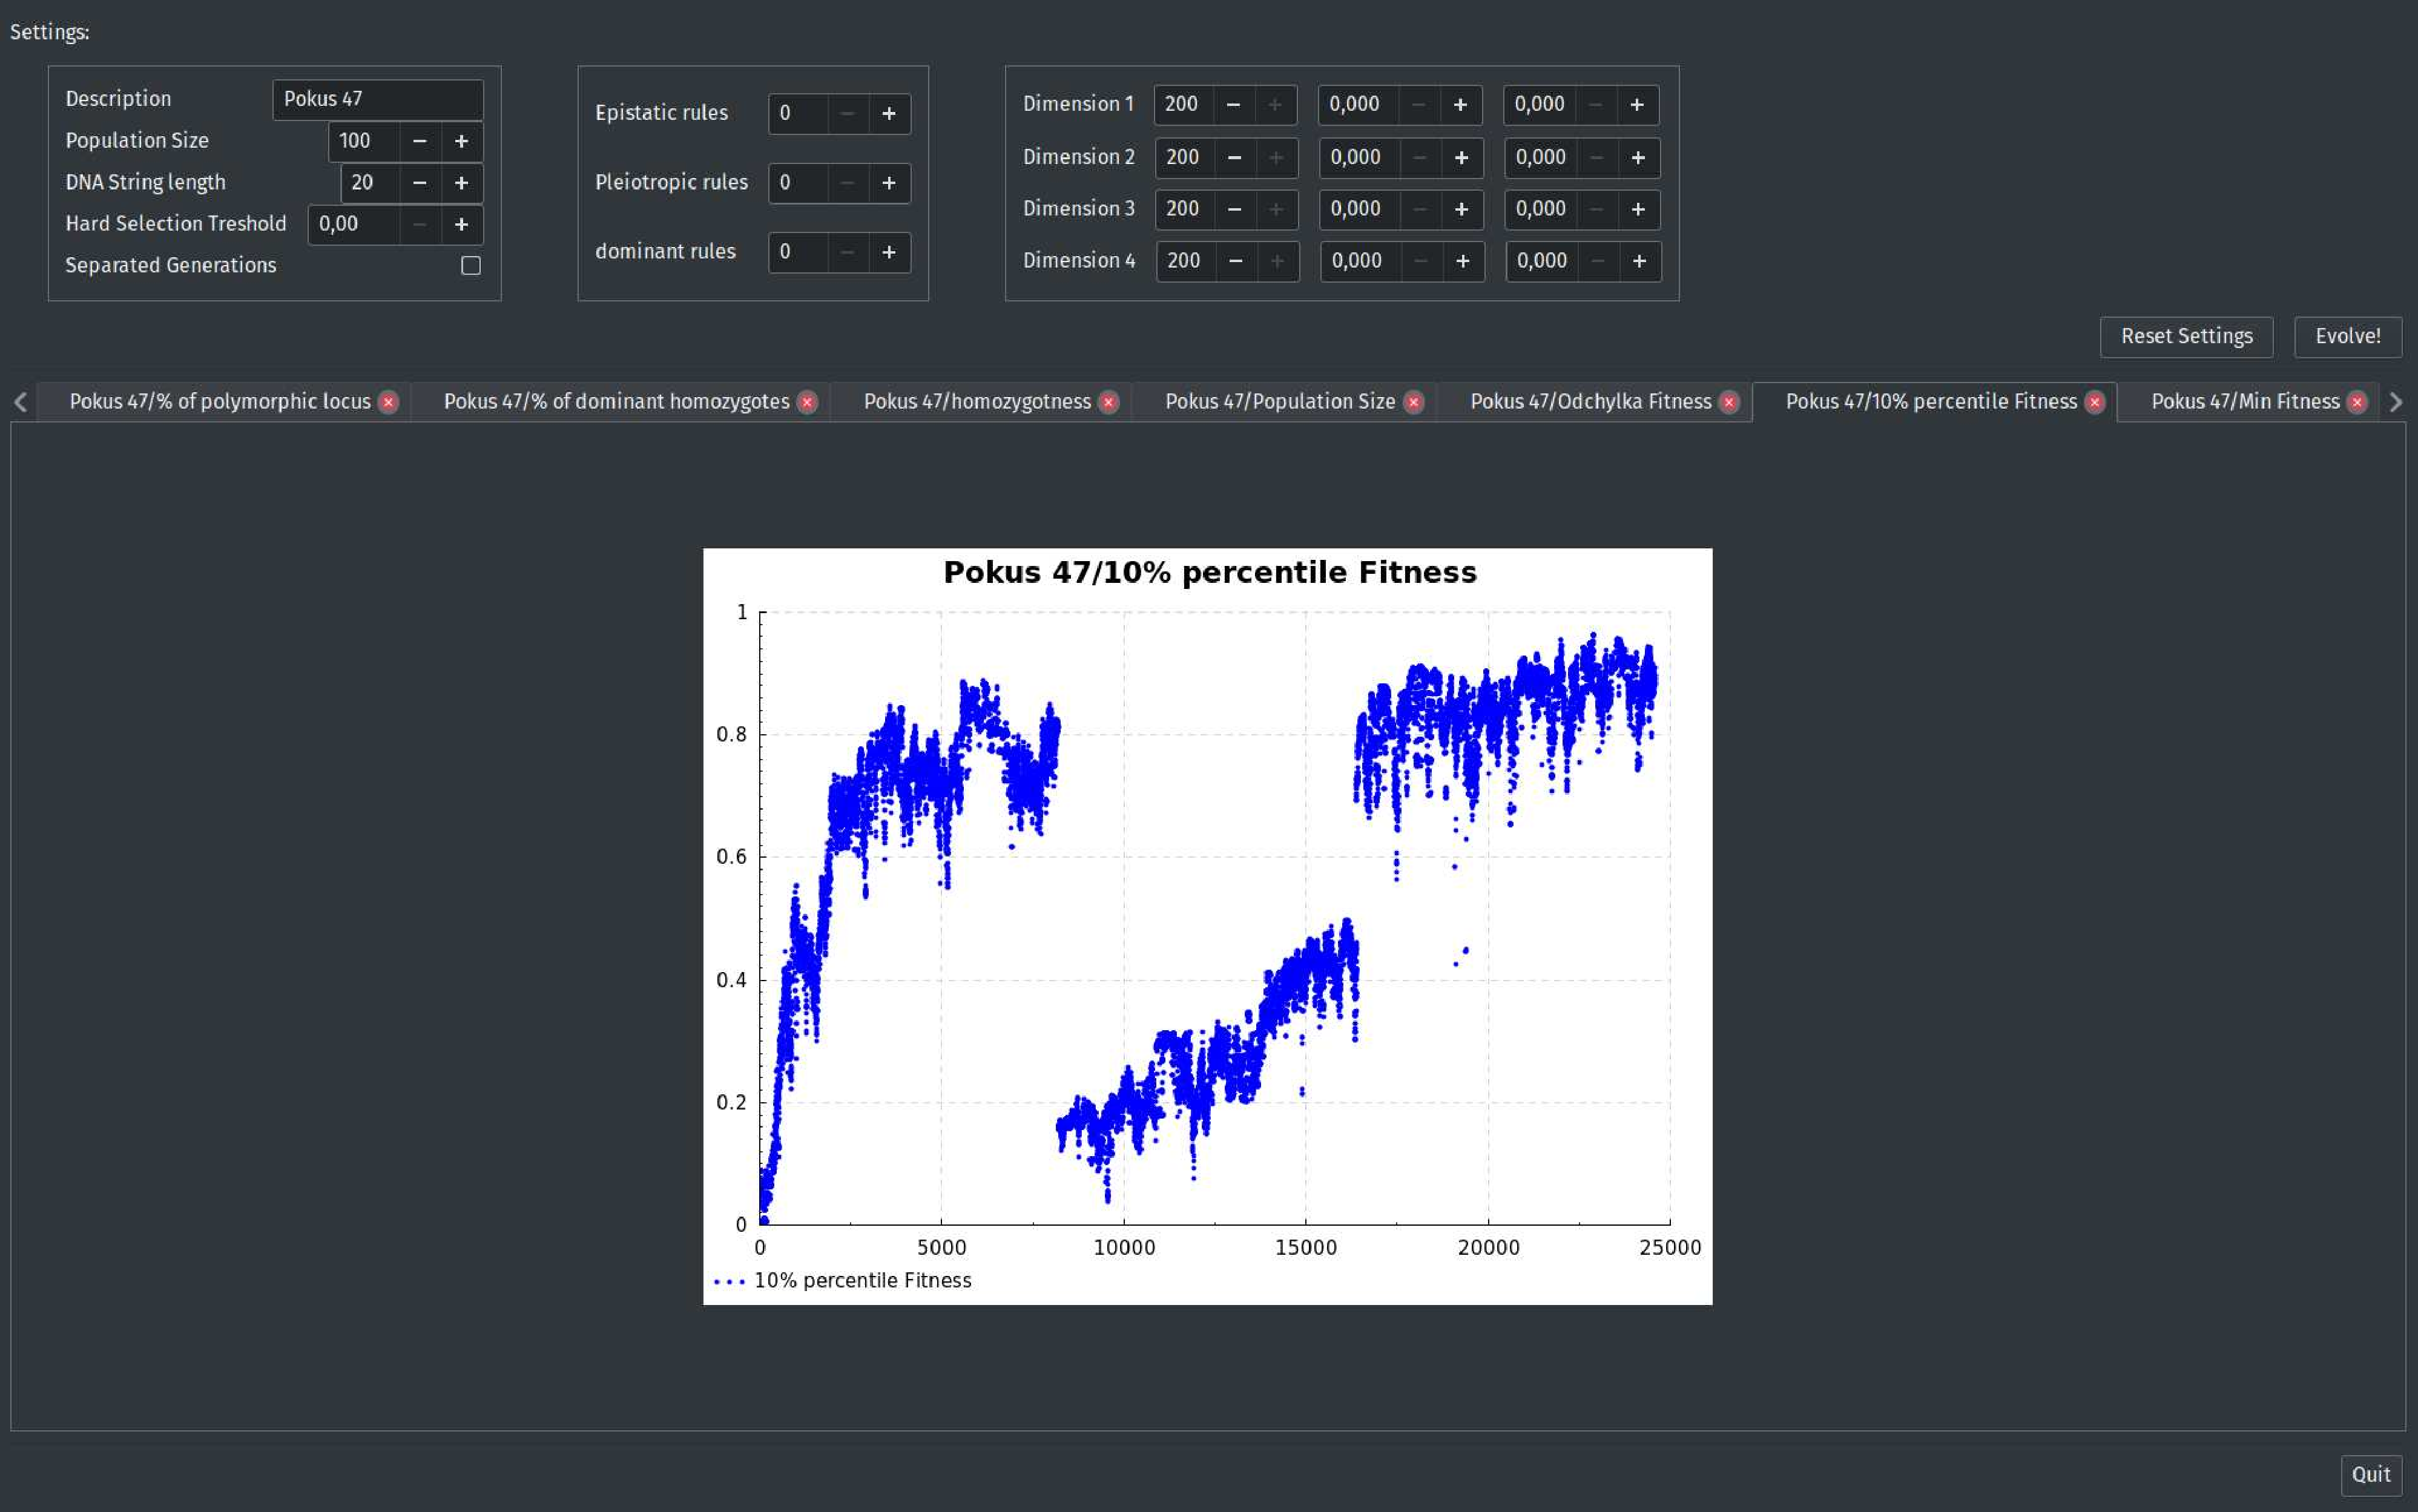
\includegraphics[totalheight=8cm]{img/Screenshot.pdf}
    \caption{\textit{FrozenBeagleSimulation} screenshot}
\label{fig:FrozenBeagleScreenshot}
\end{figure}


\textit{fbeagle} je vhodný pro dávkové zpracování, které spouští mnoho simulací se stejnými parametry, které se liší
počátečním \textit{seedem} generátoru pseudonáhodných čísel. Jeho výstupem je sada statistik pro jednotlivé simulace,
které je možné dále analyzovat a zpracovávat.

Parametry \textit{fbeagle} jsou zdokumentovány v \ref{sec:parameters}.

Na adrese \url {https://github.com/satai/FrozenBeagle} jsou volně k dispozici zdrojové texty včetně jednotkových testů
a kompletní historie ve VCS git. Jsou poskytnuty pod otevřenou trojsložkovou BSD licencí. V přiloze XXX jsou
zdokumenotovány informace, které by měly postačit k přeložení \textit{fbeagle} z těchto zdrojových textů
a jeho spuštění a reprodukování výsledků.

\begin{tcolorbox}[ title={Reprodukovatelnost v počítačových simulacích}
                 , breakable
                 ]
Reprodukovatenlost počítačových simulací by zdánlivě mělo být triviální téma. Počítače jsou
deterministické,\footnote{
Nebudu se snažit předstírat, že očekávám, že by mi to čtenář, který někdy použil reálný počítač, uvěřil, ale
taková je všeobecně opakovaná teorie.
} takže překlad zdrojových textů do spustitelného programu i následný běh tohoto
programu je deterministický a dá pro stejné parametry stejné výsledky.

To bohužel naráží na problémy čistě náhodné (například \uv{náhodné} změny hodnot v paměti
nejsou podle XXX zas tak neobvyklé), ale i systematické.

Praxe ukázala, že zajistit už jen zajistit překlad programu na vždy stejný spustitelný kód není zcela triviální (XXX).
Vyžaduje to, mimo jiné, že jsou ke každému překladu k dispozici vždy stejné nástroje (překladač, linker,
knihovny\ldots) a že překlad nezávisí například na aktuálním času, zvoleném jazyce, jménu počítače nebo přihlášeného uživatele.

Pro Haskell zajišťuje vždy stejnou verzi nástrojů a knihoven nástroj stack(XXX) a jeho systém
LTS (Long Time Support) snapshotů - repository zafixovaných verzí závislostí, u kterých je
otestováno, že jsou vzájemně kompatibilní. Na rozdíl od dříve užívané kabaly (XXX), kde překlady
závisely na okamžitém stavu počítače, je podstatně pravděpodobnější, že stejný projekt vygeneruje
stejný (a tedy i stejně se chovající) program na různých počítačích nebo na stejném počítači v různých
okamžicích.

Obdobné problémy se týkají i následného běhu simulací.

I když stochastická simulace nepoužívá náhodná čísla, ale dělá rozhodnutí pseudonáhodá na základě zadané inicializace
(\textit{seedu}), je i zde prostor pro nedeterminismus. Naštěstí je \textit{fbeagle} velké části zdrojů
nedeterminismu (časování, dělení dat v distribuovaném prostředí\ldots) ušetřen, protože funguje jako
jednoduchý dávkový program bez složitého I/O, threadů, distribuování výpočtu a synchronizací.
\end{tcolorbox}



Bla, bla. XXXXX

K sazbě byl použit systém \TeX se sadou maker \LaTeX a za použití fontů Latin Modern.

\section{Statistická analýza}

\subsection{Popisná statistika}

Pro každou simulaci a pro každý úsek simulace (první období s prvním optimem,
období s druhým optimem a závěrečné období s původním optimem) spočte \textit{fbeagle} několik statistik.

Nejjednodušší je zda populace tento úsek přežila a nebo nejpozději v něm vyhynula
(t.j. velikost populace klesla v průběhu daného úseku nebo některého předchozího úseku na nulu).

Jak úspěšně se populace v dané simulaci přizpůsobila aktuálním podmínkám, tedy jak se jedinci přiblížili k optimu,
reprezentují dvě statistiky - maximum z průměrné fitness pro dané období (pro populaci je v každém kroku
spočítána průměrná fitness a z těchto průměrů je vzato maximum - to vyjadřuje, jak nejblíže se v daném období podařilo
populaci přiblížit k optimu) a maximum z desetiprocentního percentylu fitness pro dané období.
Maximum desetiprocentního percentylu pro dané období postihuje blízkost optimu pro
málo přizpůsobené jedince v dané populaci. Percentyl je v dané situaci výstižnější statistika než minimum - to může
být výrazně ovlivněno náhodou, kdy mutace vytvoří nereprezentativního jedince fenotypem vzdáleným optimu.

Jak rychle populace reaguje na nové podmínky je měřeno směrnicí průměrné fitness v počátečním úseku daného období.
Úsek má délku 127 kroků simulace. Směrnice je tedy rozdíl průměrné fitness v kroku č. 128 a v prvním kroku daného
období vydělený 128.

\subsection{Testování hypotéz}

Hypotézy

- rychleji vymiraji, zejmena po zmenach optima

- dosahuji mensich prumeru i percentylu fitness

- maji mensi smernice
